% !TeX spellcheck = en_GB
\documentclass[journal]{IEEEtran}

\renewcommand\thesection{\arabic{section}} 
\renewcommand\thesubsectiondis{\thesection.\arabic{subsection}}
\renewcommand\thesubsubsectiondis{\thesubsectiondis.\alph{subsubsection}}
\renewcommand\theparagraphdis{\arabic{paragraph}.}

%\usepackage[retainorgcmds]{IEEEtrantools}
%\usepackage{bibentry}  
\usepackage{xcolor,soul,framed} %,caption

\colorlet{shadecolor}{yellow}
% \usepackage{color,soul}
\usepackage[pdftex]{graphicx}
\graphicspath{{../pdf/}{../jpeg/}}
\DeclareGraphicsExtensions{.pdf,.jpeg,.png}

\usepackage[cmex10]{amsmath}
%Mathabx do not work on ScribTex => Removed
%\usepackage{mathabx}
\usepackage{array}
\usepackage{mdwmath}
\usepackage{mdwtab}
\usepackage{eqparbox}
\usepackage{url}
\hyphenation{op-tical net-works semi-conduc-tor}
\usepackage{graphicx}
\usepackage{notoccite}


%New from timo for project report=========================
\DeclareUnicodeCharacter{00A0}{ }
\usepackage{amssymb}

%=========================

%\bstctlcite{IEEE:BSTcontrol}
%=== TITLE & AUTHORS ====================================================================
\begin{document}

\bstctlcite{IEEEexample:BSTcontrol}
    \title{Generation of Real Looking Images Using GANs 
     }

  \author{\textbf{BOHNSTEDT Timo, B.Sc.} \\ Friedrich Alexander University \\ \textit{timo.bohnstedt@fau.de}% \\ <-this % stops a space
}

% The paper headers
\markboth{Final Paper for the Machine Learning in the Industry 4.0 Seminar at the FAU 
}{Roberg \MakeLowercase{\textit{et al.}}}


% ====================================================================
\maketitle
% === ABSTRACT 
\begin{abstract}
%\boldmath
Automatic image generation is a complex task with many applications in several domains such as policing (e.g. generating portraits from the description), styling and entertainment. In this project, advanced versions of Generative Adversarial Networks (GANs) are used to generate real looking images. A conditional GAN (cGAN) is used as a prototype, followed by an evaluation with visual examination, k-nearest-Neighbours (kNN) and  Fréchet Inception Distance (FID). The evaluation indicates that a cGAN can generate realistic images of handwritten digits. Whereas, the discussion shows that more work must be done to create realistic images from datasets which contains larger and more complex images. 
\end{abstract}

% === KEYWORDS 
\begin{IEEEkeywords}
Machine Learning in the Industry 4.0, EDA, Data Analytics, FAU, Python, GANs, cGANs
\end{IEEEkeywords}

\IEEEpeerreviewmaketitle

% === I. Project background and motivation
\section{Introduction}
\IEEEPARstart{G}{}enerative Adversarial Networks (GANs) have been getting a lot of attention recently. They are used for different tasks, such as image-to-image translation where images can be transferred from one domain to another, text to image translation and super-resolution. 
GANs are introduced as an unsupervised learning model, trained on data without labels. The model learns to map noise to images reassembling examples from the training set.

There exist several challenges to model distributions in a stable and discriminative way. The two main issues are a slow training process and mode collapse.

Optimizing a GAN can be treated as optimizing the JS-divergence. This leads to the problem of vanishing gradients in early training if the original dataset and the generated dataset are very different. To encounter this problem, Goodfellow et al. suggested to use another loss function. That means optimizing a GAN can no longer be treated as optimizing the JS-divergence, and it shrinks the probability of suffering from vanishing gradients. The solution works in practice despite a scientific discourse. This is why, in this paper, we focus on mode collapse. 

Mode collapse means a lack of image diversity. Instead of reproducing all classes, one or more modes can be observed in the generated data set. This means that one or more classes occur most frequently in the data set. It would be desirable if there is no mode, i.e. no class that occurs more often in relation to all other classes. 

There are versions of GANs that can use additional information as input, such as conditional GANs (cGANS). Research suggests to use cGANS to get a higher chance that mode collapse does not appear  \cite{DBLP:journals/corr/IsolaZZE16,DBLP:journals/corr/SalimansGZCRC16}. 

Deep networks require a large amount of examples for successful training. Because data acquisition is usually quite  time-consuming, we want to reduce this effort by generating real world images from noise. As such we have the following two research questions:\\

\begin{quote}
	\itshape{\begin{itemize}
			\item Is it possible to generate real-looking images?
			\item Is it possible to introduce enough inter-class variance for training?
		\end{itemize}}
\end{quote}

This paper focuses on answering both questions.

% === II. Procedural Method==================================== 
\section{Methods}
GANs are a framework for estimating generative models via an adversarial process, in which two models get trained simultaneously. A generative model \boldmath{\(G\)} that captures the data distribution and a discriminative model \boldmath{\(D\)} that estimates the probability that a sample is drawn from the training data rather than from \boldmath{\(G\)} \cite{Goodfellow-et-al-2016}. Simplified, the generator tries to produce data that comes from some probability distribution. 

Figure \ref{fig:gan-forward-step} highlights by example how the forward step works.\footnote{The image is retrieved from the TensorFlow website. It is part of an intuitive example of how to interpret GANs \cite{tensorflow2020}}. 

Mathematically this problem can be described as solving a two-player min-max game. The problem is divided into three parts:

\begin{enumerate}
	\item Maximize the chance to recognize real images as real.
	\item Maximize the chance to recognize fake images as fake.
	\item Optimize \boldmath{\(G\)} such that it fools \boldmath{\(D\)} the most.\\
\end{enumerate}

The first two steps can be summarized with the following equation where \boldmath{\(D(x)\) outputs a value indicating the chance that \boldmath{\(x\) is a real image \cite{goodfellow_generative_2014}:
		
\begin{equation}
\begin{split}
\thinspace \underset{D}{max} \thinspace V(D) &= \mathbb{E}_{x \sim p_{data}(x)}[log \thinspace D(x)]\\
& + \mathbb{E}_{z \sim p_{z}(z)}[log(1 - D(G(z)))]
\label{eq:value_func}
\end{split}
\end{equation}

Therefore \(x\) stands for the generated images, \(V\) is the value function of \(D\) and \(z\) is noise which is transformed by the network into real-looking images. Furthermore, \(p_{data}\) means that we sample \(x\) from the data set of the original images and \(p_{z}\) means we sample noise \(z\) from a distribution which generates random noise.

Note that the first addend is to recognize real images better and the second addend is to recognize fake images better. So, the objective function of \boldmath{\(G\)} can be described as follows:

\begin{equation}
\begin{split}
\thinspace \underset{G}{min} \thinspace V(G) = \mathbb{E}_{z \sim p_{z}(z)}[log(1 - D(G(z)))]
\label{eq:value_func}
\end{split}
\end{equation}

By using gradient decent as an optimization technique and using the chain rule to get the derivates of the objective functions one step of particular training involves the following steps \cite{goodfellow_generative_2014}:

\begin{itemize}
	\item Sample a mini batch of \boldmath{\(m\)} noise vectors \( \{z^{(1)},\dots,z^{(m)}\} \).
	\item Sample a mini batch of m \boldmath{\(m\)} training samples \( \{x^{(1)},\dots,x^{(m)}\} \).
	\item Update  \boldmath{\(D\)}  by doing one gradient descent step on its loss function:
	\begin{equation}
	\begin{split}
	J_D &= - \frac{1}{m} \sum_{i=1}^{m} \Big[log \thinspace D\big(x^{(i)}\big)\\
	&+log\big(1 - D\big(G\big(z^{(i)}\big)\big)\big)\Big]
	\label{eq:J_D}
	\end{split}	
	\end{equation}
	\item Update  \boldmath{\(G\)}  by doing one gradient descent step on its loss function: 
	\begin{equation}
	J_G = - \frac{1}{m} \sum_{i=1}^{m} \Big[log \thinspace D\big(G\big(z^{(i)}\big)\big)\Big]
	\label{eq:J_G}
	\end{equation}
\end{itemize}

The cGAN can be constructed by merely feeding the labels \boldmath{\(y\)} into both the generator and discriminator \cite{DBLP:journals/corr/MirzaO14}.

The generator \boldmath{\(G\)} and the discriminator \boldmath{\(D\)} are now conditioned with  additional information \boldmath{\(y\)}. So the steps of the training are now as follows \cite{DBLP:journals/corr/IsolaZZE16}:

\begin{itemize}
	\item Sample a mini batch of \boldmath{\(m\)} noise vectors \( \{z^{(1)},\dots,z^{(m)}\} \).
	\item Sample a mini batch of m \boldmath{\(m\)} training samples \( \{(x^{(1)},y^{(1)}),\dots,(x^{(m)},y^{(m)})\} \).
	\item Update  \boldmath{\(D\)}  by doing one gradient descent step on its loss function:
	\begin{equation}
	\begin{split}
	J_D &= - \frac{1}{m} \sum_{i=1}^{m} \Big[log \thinspace D\big(x^{(i)}, y^{(i)}\big)\\
	&+log\big(1 - D\big(G\big(z^{(i)},y^{(i)}\big),y^{(i)}\big)\big)\Big]
	\label{eq:J_D}
	\end{split}	
	\end{equation}
	\item Update  \boldmath{\(G\)}  by doing one gradient descent step on its loss function: 
	\begin{equation}
	J_G = - \frac{1}{m} \sum_{i=1}^{m} \Big[log \thinspace D\big(G\big(z^{(i)},y^{(i)}\big),y^{(i)}\big)\Big]
	\label{eq:J_G}
	\end{equation}
\end{itemize}

We use a dataset of handwritten digits as training data, which is produced by the Mixed National Institute of Standards and Technology (MNIST). This dataset is a good fit because of its sheer size, allowing GANs to work efficiently. This dataset contains 50,000 training images and 10,000 testing images, formatted as 28 \(\times\) 28 pixel monochrome images. Figure \ref{fig:mnist-example} shows the images contained in this dataset.

\begin{figure}[htp]
	\centering
	\fbox{\includegraphics[width=0.9\linewidth]{img/gan-forward-step}}
	\caption{
		Two models are trained simultaneously by an adversarial process. A generator ("the artist") learns to create images that look real, while a discriminator ("the art critic") learns to tell real images apart from fakes \cite{tensorflow2020}.
	}
	\label{fig:gan-forward-step}
\end{figure}


The overall procedure is depicted in Figure \ref{fig:cdcgan-forward-step}. The left column depicts the generator network \boldmath{\(G\)}, the right column the discriminator network \boldmath{\(D\)}.

\begin{figure}[htp]
	\centering
	\fbox{\includegraphics[width=0.9\linewidth]{img/mnist-example}}
	\caption{
		A few examples of the so-called MNIST dataset which contains 60,000 images of handwritten digits.
	}
	\label{fig:mnist-example}
\end{figure}

First, the noise and the labels are passed to \boldmath{\(G\)}. The different layers of the network perform dense and reshape operations before the vectors are concatenated. Finally,  \boldmath{\(G\)} produces images at the same size as the original images. Afterwards, a real image and the generated image get passed to \boldmath{\(D\)}, which uses dense and reshape operations as well. Finally, \boldmath{\(D\)} \textit{decides} whether or not this is a real or a generated image, as can be observed on the bottom right in Figure \ref{fig:cdcgan-forward-step}. 

Precisely, the generator of the DCGAN uses upsampling layers to produce an image from random noise. It starts with a dense layer that takes this seed as input, then \boldmath{\(G\)} upsamples serval times until it reaches the desired image size. The Network uses a leaky ReLU activation function for each layer, except the output layer which uses tanh. The generator network of the DCGAN is a CNN-based image classifier. It uses two convolutional layers, followed by a dropout layer. \boldmath{\(D\)} uses the leaky ReLU activation function as well. 

The generator network of the cDCGAN prepares the input and the labels by bringing the data into the desired form. Therefore it uses two dense, and two reshape layers each, before it gets concatenated. Then the combined input will be upsampled as in the generator network of our DCGAN.

The discriminator model of the cDCGAN is also a CNN-based image classifier. It uses two convolutional layers and two pooling layers for the generated input images . For the labels \boldmath{\(G\)} uses two dense layers. After the two inputs get through the mentioned layers, they will be concatenated as well. 

We use a training size of 50,000 images, a batch-size of 128 images, 20 epochs and we use the Adam optimizer.


\begin{figure}[htp]
	\centering
	\fbox{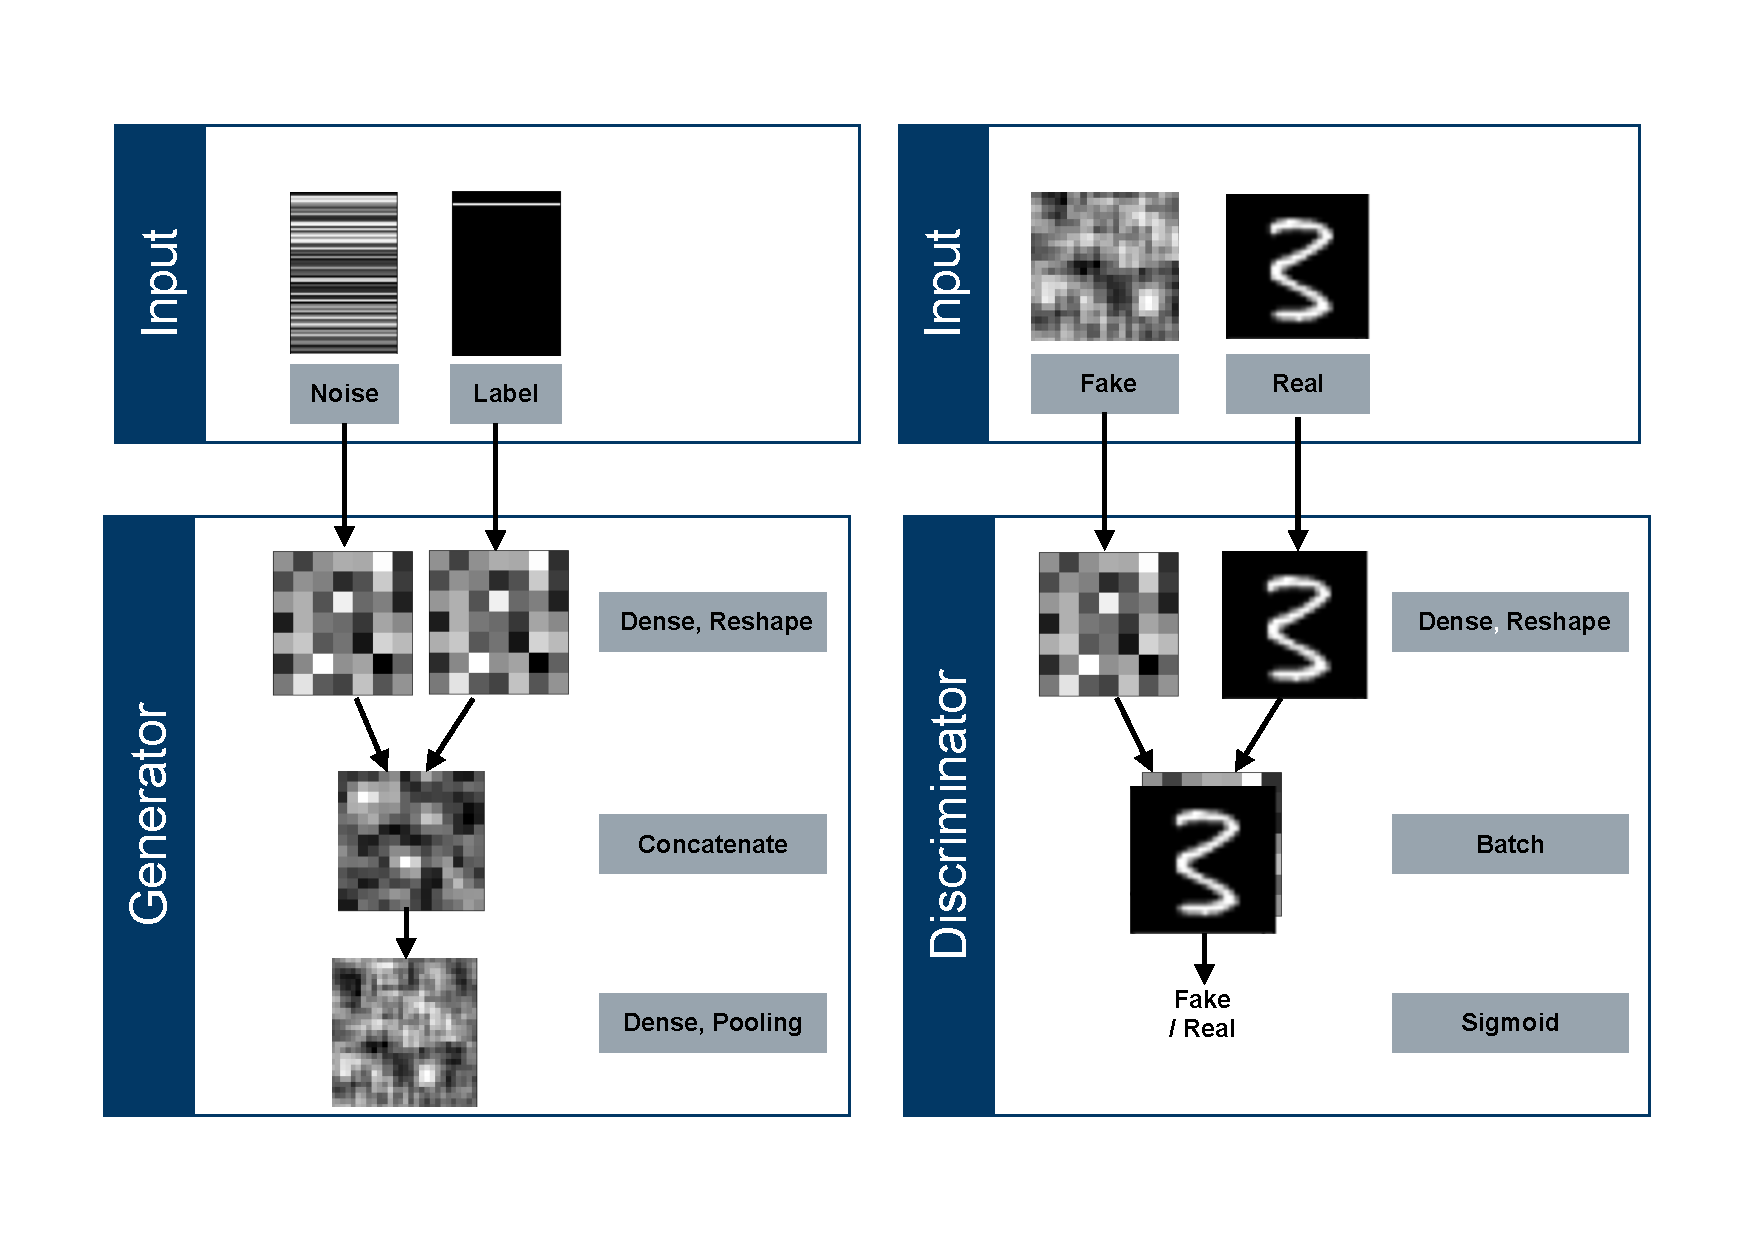
\includegraphics[width=0.9\linewidth]{img/cdcgan-forward-step}}
	\caption{
		Two distinct inputs get fed into the generator to create images. Different dense, reshape operations and finally the concatenation of the images transforms the images such that the model can be trained by using gradient decent as optimization technique.
	}
	\label{fig:cdcgan-forward-step}
\end{figure}

GAN training faces some problems when it comes to generating real-looking images. Therefore, a conditional Deep Convolutional GAN (cDCGAN) offers a more stable training process. The generator of the DCGAN uses the transposed convolution technique to perform up-sampling of 2D images, such that the cDCGAN is considered as a better fit when it comes to generating real-looking images. Figure \ref{fig:cdcgan-backward-step} highlights the data-flow and the gradients used for the backpropagation \cite{goodfellow_generative_2014}.  After performing on a particular step of gradient decent, a maximum error is used to adjust the weights within the layers of \boldmath{\(G\)}. Therefore a minimum error is used to adjust the weights within the layers of \boldmath{\(D\)}. 

\begin{figure}[htp]
	\centering
	\fbox{\includegraphics[width=0.9\linewidth]{img/cdcgan-backward-step}}
	\caption{
		The Figure summarizes the data-flow and the gradients used for the backpropagation \cite{goodfellow_generative_2014}. 
	}
	\label{fig:cdcgan-backward-step}
\end{figure}


\boldmath{\(G\)} is implemented such that \(-log \thinspace D(G(z))\) instead of \(log(1 - D(G(z)))\) is minimized as suggested in the original GAN paper \cite{goodfellow_generative_2014}. It ensures stronger gradients for \boldmath{\(G\)} early in training while keeping the same fixed point dynamics of \boldmath{\(G\)} and \boldmath{\(D\)}, as shown in the value function (Equation 2).

The performance of \boldmath{\(G\)} compared to \boldmath{\(D\)} is usually poor in the early stages of the training process. That means \boldmath{\(D\)} can easily distinguish fake examples from real images. Therefore the learning of \boldmath{\(D\)} is implemented such that it learns slower, which is done by running more than one training step for \boldmath{\(G\)} for every step of \boldmath{\(D\)} and lowering the learning rate of \boldmath{\(D\)}.

GANs and cGANs stipulate a high-level framework with a lot of freedom in designing its various components. The prototype which will be used in order to find answers to the research question uses a so-called conditional deep convolutional neural network (cDCGAN) and uses the hyperparameters suggested by Isola et al. \cite{DBLP:journals/corr/IsolaZZE16}.  To set a baseline within the evaluation a DCGAN will be implemented as well. 

\section{Results} 

Great care must be taken when it comes to presenting and evaluating the results of any GAN. The objective functions presented in the methods section can not tell necessarily the quality of the image. Furthermore, there is not an exact definition of good quality. The objective functions for G and D are relative measurements. Their results indicate the performance with respect to each other. For this reason, we consider a visual examination, followed by quantitative measurements. Furthermore, quantitative measurements, such as the inception score and the Fréchet Inception Distance (FID), can be combined with a qualitative evaluation approach to provide a robust evaluation \cite{DBLP:journals/corr/abs-1802-03446,DBLP:journals/corr/IsolaZZE16}.

When it comes to the evaluation of the results visual examination, k Nearest Neighbour (kNN) and the FID is used.

FID is a metric that calculates the distance between feature vectors calculated for real and generated images.

The score summarizes how similar the two groups are in terms of statistics on computer vision features of the raw images calculated using a CNN-based model which can be used for image classification. Lower scores indicate the two groups of images are more similar, or have more similar statistics, with a perfect score being 0.0, meaning that the two groups of images are identical.
 \cite{DBLP:journals/corr/HeuselRUNKH17}.

\begin{figure}[htp]
	\centering
	\fbox{\includegraphics[width=0.9\linewidth]{img/visual-fid-gan-cgan}}
	\caption{
		 Images generated by the DCGAN (left) and the cDCGAN (right) and their corresponding FID-scores show that the images generated by DCGAN are more realistic. 
	}
	\label{fig:visual-fid-gan-cgan}
\end{figure}

Figure \ref{fig:visual-fid-gan-cgan} highlights the result of the visual examination. The images produced by the cDCGAN (right) look quite real, whereas the images from the DCGAN have just one mode (left). The FID score for the DCGAN and the cDCGAN is also shown in Figure \ref{fig:visual-fid-gan-cgan}. The score indicates that the results from the visual examination are correct because the score of the DCGAN generated images is proportionally higher in comparison with the cDCGAN generated images. Figure \ref{fig:knn-gan-cgan} highlights the results of the kNN approach. In the dataset generated by the DCGAN, just on mode appears if we search for the nearest neighbour in the original dataset. Whereas if we use the dataset generated by the cDCGAN, the nearest neighbours have no mode. 

\begin{figure}[htp]
	\centering
	\fbox{\includegraphics[width=0.9\linewidth]{img/knn-gan-cgan}}
	\caption{
		 The evaluation with the kNN shows that just one digit in the original dataset is close to the generated images.
	}
	\label{fig:knn-gan-cgan}
\end{figure}

Figure \ref{fig:evaluation-training-proces}} shows that the loss fluctuates more within the cDCGAN training in comparison to the DCGAN training procedure. At the same time, the loss curves from the cDCGAN decrease more within the final epochs. The GAN trained for 3.32 seconds per epoch on average, whereas the cDCGAN trained for 53.02 seconds per epoch on average. Note that the overall loss for cDCGAN is lower than cDCGAN. Secondly, it could be that with much longer training, CDCGAN could have similar loss, but with much longer training time. Furthermore, the loss of the generator and the discriminator decrease in the cDCGAN training procedure compared to the CGAN.

\begin{figure}[htp]
	\centering
	\fbox{\includegraphics[width=0.9\linewidth]{img/evaluation-training-process.png}}
	\caption{
		The loss of \boldmath{\(G\)} and \boldmath{\(D\)} compared for a GAN (left) and a cDCGAN (right) architecture. 
	}
	\label{fig:evaluation-training-proces}
\end{figure}

\section{Discussion}

As shown above, cGANs have performed remarkably well on the task of generating realistic images. However, as the complexity rises the results are getting surprisingly worse. For example, if the dataset contains photographs from objects on a conveyor belt, the generated images are not realistic at all. It is not even necessary to go towards visual examination because the results are so obvious. An example can be seen in Figure \ref{fig:cdcgan-results-compared-madi-dataset}. Note two more dense layers and additional training time is added to ensure that the training process can be started.

\begin{figure}[htp]
	\centering
	\fbox{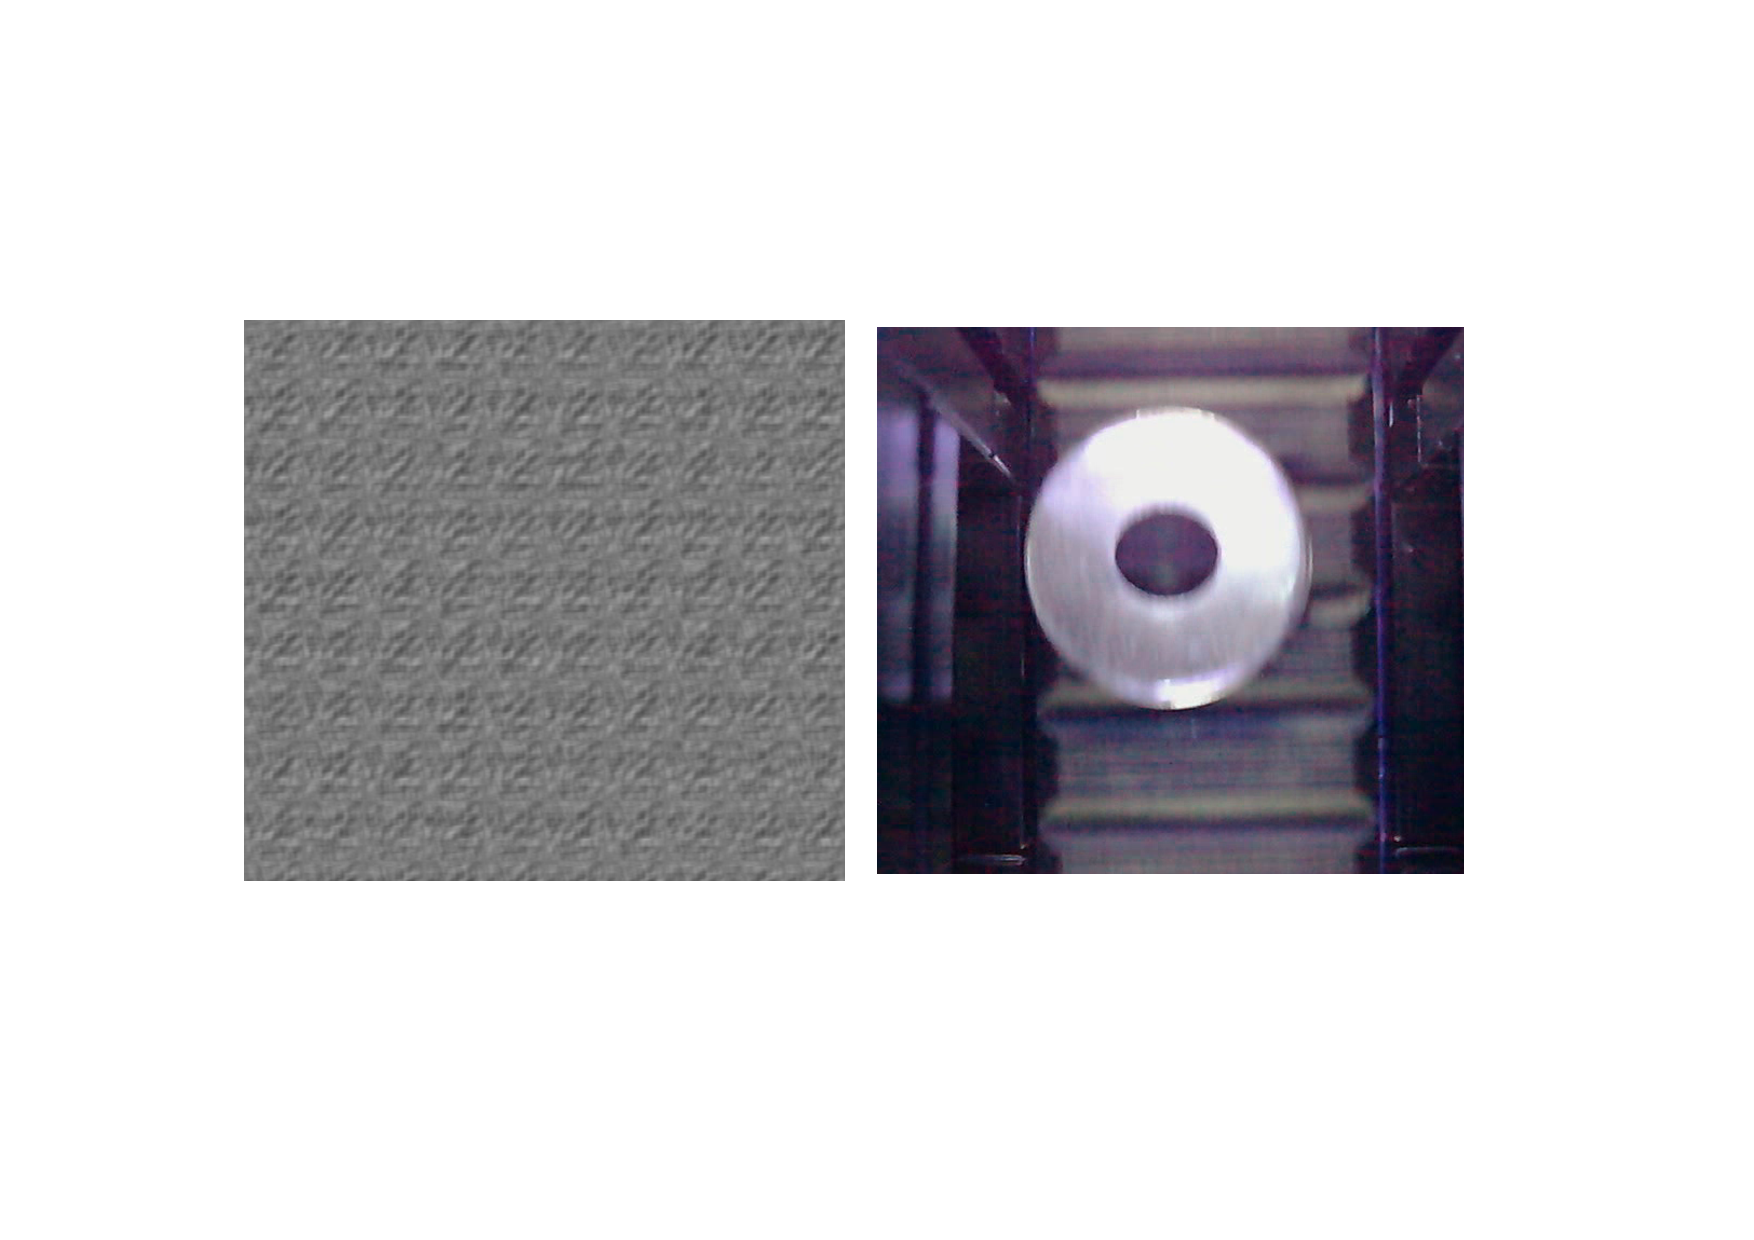
\includegraphics[width=0.9\linewidth]{img/cdcgan-results-compared-madi-dataset.png}}
	\caption{
		The image shows the result (left) while using another dataset (right).
	}
	\label{fig:cdcgan-results-compared-madi-dataset}
\end{figure}

Salimans et al. suggest an iterating process in order to find the most suitable values for the following hyperparameters: \cite{DBLP:journals/corr/SalimansGZCRC16}:
\begin{itemize}
\item The discriminator’s optimizer.
\item The learning rate.
\item Dropout probability.
\item Batch size.
\end{itemize}

Therefore Goodfellow suggested to try different loss functions in order to significantly speed up the training process and thus to decrease the loss in a shorter amount of time \cite{DBLP:journals/corr/Goodfellow17}. 

Unrolled GANs are another method to prevent a GAN and a cDCGAN for mode s collapse \cite{DBLP:journals/corr/Goodfellow17}. It lowers the chance that the generator is overfitted for a specific discriminator by defining the generator objective with respect to an unrolled optimization of the discriminator.

Figure \ref{fig:cdcgan-results-compared-madi-dataset} shows that the performance of the cDCGAN can be strongly affected by the training set. All improvements mentioned above could help to improve the results of a future scenario. Within this scenario, we could try to use another dataset with larger images and the mentioned approaches to improve the training procedure of a DCGAN and cDCGAN.
 
\section{Conclusion}
Image generation conditioned on labels is a complex task that requires a model to learn not only the general data distribution for images, but also label embeddings for each individual class. It can be concluded from the results that well-designed cDCGANs can perform admirably well on this very complex task. Provided high-quality input data, these cGANs can be trained so that the combination of a conditional and the noise vector (\(z\)) actually can generate images of handwritten digits. It is planned to expand this work in two directions. First, improving the training process by tuning the hyperparameters and secondly supporting any combination of training images and training labels. 


\ifCLASSOPTIONcaptionsoff
  \newpage
\fi
\bibliographystyle{IEEEtran}
\bibliography{IEEEabrv,Bibliography}

\vfill
\end{document}